%! Author = wolfram_e_laube
%! Date = 07.04.24

% Preamble
\documentclass{beamer}

\usetheme{Madrid} % This is a simple and clean theme, but you can change it to other themes like: Berlin, Warsaw, etc.

\title{Label Characteristics Analysis}
\subtitle{Grouping and Class Balance in Speech Command Recognition}
\author{Team Park: W. Laube, D. Hörtenhuber, O. König}
\institute{JKU \\ MLPC}
\date{\today}

\begin{document}

\begin{frame}
  \titlepage
\end{frame}

\begin{frame}{Introduction}
  \begin{itemize}
    \item \textbf{Purpose of Analysis:} Optimize grouping and interpretation of speech commands for improved system interaction.
    \item \textbf{Importance of Effective Grouping:} Properly categorized commands enhance model accuracy and user experience.
    \item \textbf{Examining Class Balance:} Balanced datasets lead to robust models, reducing bias and improving performance.
    \item \textbf{Relevance to Model Training:} Direct impact on training strategies, affecting the efficiency and effectiveness of the learning process.
  \end{itemize}
\end{frame}

\begin{frame}{Grouping Strategy and Rationale}
  \begin{itemize}
    \item \textbf{Semantic Similarity and Contextual Use:}
      \begin{itemize}
        \item \textit{Functional Groupings}: Group labels by functionality to enhance model training and prediction accuracy.
        \item \textit{Contextual Groupings}: Align groupings with typical usage scenarios to reflect real-world applications.
      \end{itemize}
    \item \textbf{Rationale:}
      \begin{itemize}
        \item \textit{Enhanced Recognition}: Facilitate more precise command recognition and reduce misinterpretations.
        \item \textit{User Interaction}: Improve user experience by responding accurately to context-driven commands.
      \end{itemize}
    \item \textbf{Visualization}:
      \begin{figure}
        \centering
        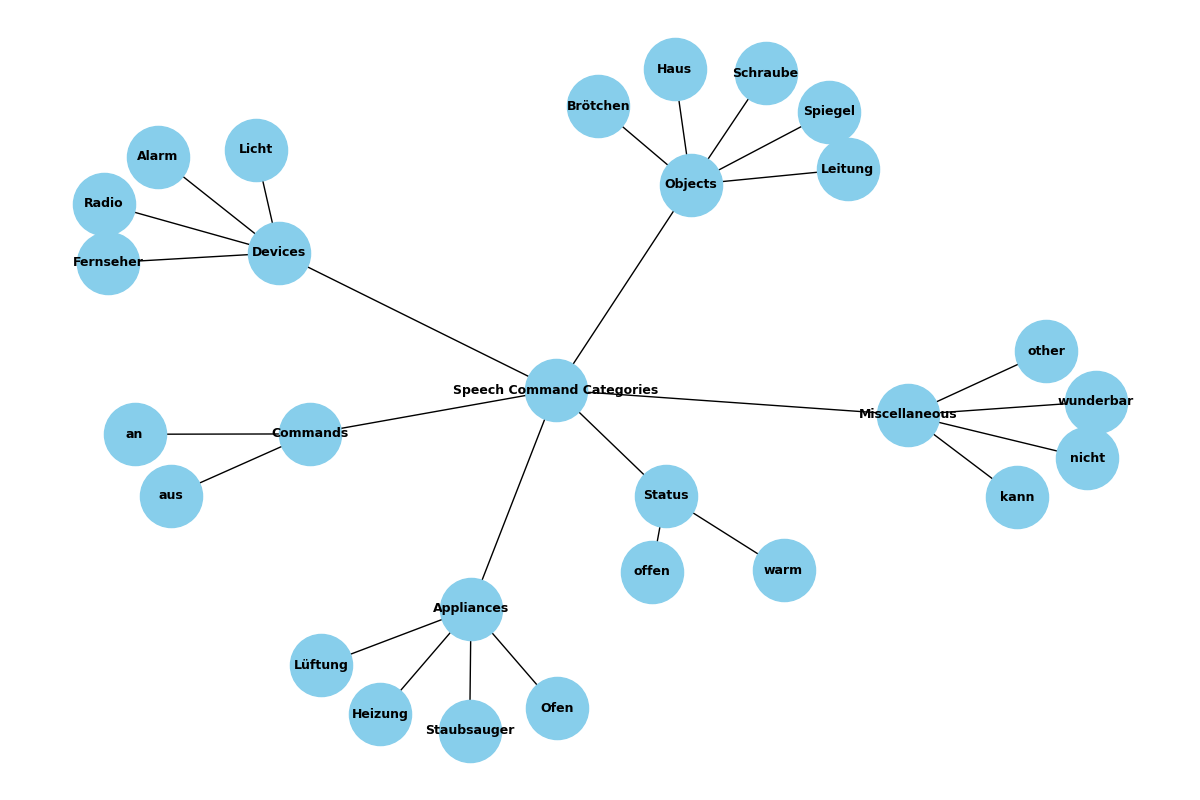
\includegraphics[width=0.7\textwidth]{fig/mindmap_command_grouping} % Ensure the path and filename are correct
        \caption{Categorization of Speech Commands}
        \label{fig:grouping}
      \end{figure}
  \end{itemize}
\end{frame}

\begin{frame}{Class Balance Analysis}
  \begin{itemize}
    \item \textbf{Presentation of Data:} Show the distribution of labels across different groups to identify balance and imbalances.
    \item \textbf{Visualization:}
      \begin{figure}
        \centering
        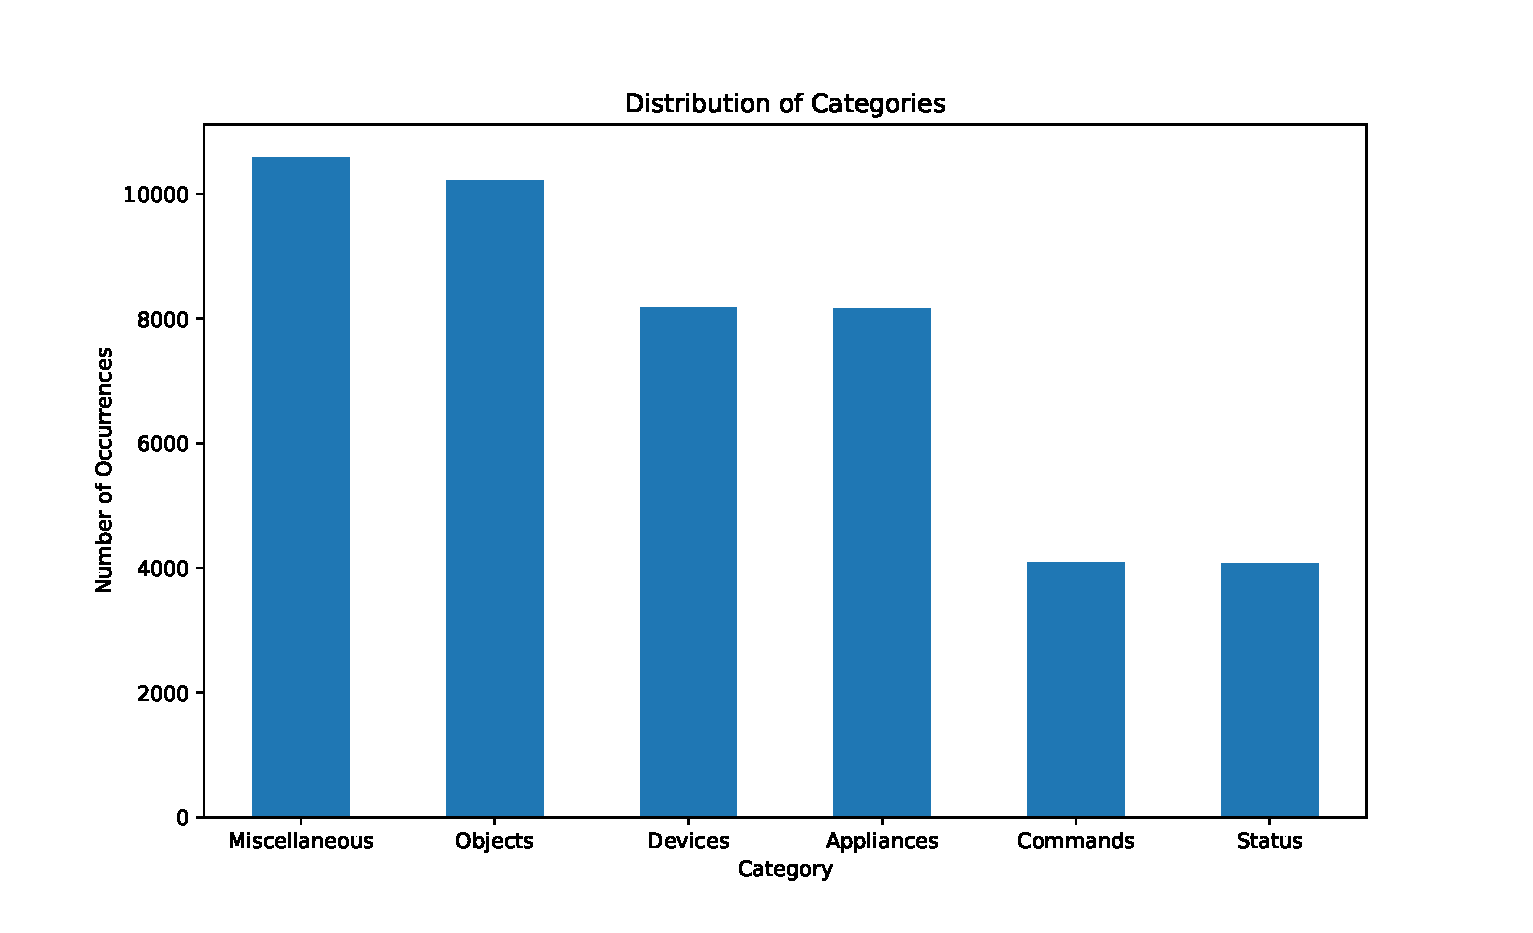
\includegraphics[width=0.75\textwidth]{fig/categories_dist} % Ensure the path and filename are correct
        \caption{Distribution of Speech Commands Across Groups}
        \label{fig:class_balance}
      \end{figure}
    \item \textbf{Highlight Imbalances:} Discuss the impact of observed imbalances on model training, such as the potential for overfitting to more common classes and underperformance on rarer ones.
  \end{itemize}
\end{frame}

\begin{frame}{Managing Class Imbalance in Speech Command Recognition}
  \begin{itemize}
    \item \textbf{Impact of Imbalance:}
      \begin{itemize}
        \item Model bias towards overrepresented classes.
        \item Increased risk of failing to recognize critical but less common commands.
      \end{itemize}
    \item \textbf{Strategies to Mitigate Imbalance:}
      \begin{itemize}
        \item \textit{Data Augmentation:} Generate synthetic examples to enhance balance.
        \item \textit{Resampling Techniques:} Adjust the dataset by resampling classes.
        \item \textit{Adjusting Class Weights:} Modify weights during training to emphasize minority classes.
      \end{itemize}
    \item \textbf{Recommendations:}
      \begin{itemize}
        \item Select strategies based on dataset characteristics and model needs.
        \item Implement combined approaches for optimal results.
      \end{itemize}
  \end{itemize}
\end{frame}

\end{document}
